d\documentclass[letterpaper]{sig-alternate-10pt}

\usepackage{epsfig,endnotes}
%\usepackage{usenix,epsfig,endnotes}
%\usepackage{amsmath,amssymb,alltt,times,mathptmx,graphicx}
\usepackage{amsmath,amssymb,times,graphicx,amsfonts}
\usepackage{courier,subfigure,color,sped,url,wrapfig}
\usepackage{xspace}
\usepackage{balance}
\usepackage{enumitem}
%\usepackage[square,comma,numbers,sort&compress]{natbib} %REMOVED. this package setting comflict with 'sig-alternate-10pt.cls'
%\usepackage[font=sf, labelfont={sf,bf}, margin=0.5cm]{caption}
%\usepackage[labelfont={bf},margin=0.3cm]{caption}
%\usepackage{citesort}

% \usepackage[colorlinks=true, linkcolor=blue,
%               citecolor=blue, urlcolor=blue,
%               ps2pdf,                %%% hyper-references for ps2pdf
%               bookmarks=true,        %%% generate bookmarks ...
% 	      bookmarksopen=true,
%               bookmarksnumbered=true,%%% ... with numbers
%   ]{hyperref}

% \hypersetup{ pdfcreator  = {LaTeX with hyperref package},
%                pdfproducer = {dvips + ps2pdf} }
               
%\let\url\nolinkurl % because dvips cannot break url across lines
%\hypersetup{
%pdfauthor   = {},
%pdftitle    = {},
%pdfsubject  = {},
%pdfkeywords = {},
%}

\urlstyle{rm}

\usepackage{lastpage}

%%It seems these two packages must be loaded AFTER hyperref
\usepackage{algorithm}
\usepackage[noend]{algorithmic}
%\usepackage{enumitem}

%%% Local Variables:
%%% mode: latex
%%% TeX-master: "paper"
%%% End:

% Useful macros for paper writing

\definecolor{brown}{cmyk}{0,0.81,1,0.60}
\definecolor{magenta}{rgb}{0.4,0.7,0}
\definecolor{gray}{rgb}{0.5,0.5,0.5}
\definecolor{red}{rgb}{1,0,0}
\definecolor{green}{rgb}{0.5,0,0.5}
\definecolor{blue}{rgb}{0,0,1}
\newcommand{\etc}{\emph{etc.}\xspace}
\newcommand{\ie}{\emph{i.e.,}\xspace}
\newcommand{\eg}{\emph{e.g.,}\xspace}
\newcommand{\etal}{\emph{et al.}\xspace}
\newcommand{\vlc}{vlc\xspace}
\newcommand{\SNOOZE}{Snooze\xspace}
\newcommand{\snz}{Snooze\xspace}
\newcommand{\POLICE}{Police\xspace}
\newcommand{\police}{Police\xspace}
\newcommand{\Police}{Police\xspace}
\newcommand{\PSTA}{Police Station\xspace}
\newcommand{\RTH}{\textbf{A}\xspace}
\newcommand{\ISI}{\textbf{B}\xspace}
%\newcommand{\reducefiguretopvmargin}{\vspace*{0ex}}
%\newcommand{\reducefigurebottomvmargin}{\vspace*{0.0ex}}
\newcommand{\reducefigurebottomvmarginsmall}{\vspace{-3mm}}
\newcommand{\reducefigurebottomvmargin}{\vspace{-4mm}}
\newcommand{\reducefigurecaptionmargin}{\vspace{-0mm}}
\newcommand{\reduceparavmargin}{\vspace*{0.0ex}}
%\newcommand{\reduceparavmargin}{\vspace*{-2.0ex}}
\newcommand{\reducesectionvmargin}{\vspace*{0.0ex}}
%\newcommand{\reducesectionvmargin}{\vspace*{-1.0ex}}
\newcommand{\reducevmarginsmall}{\vspace*{-.5ex}}
\newcommand{\reducevmarginone}{\vspace*{-1.0ex}}
\newcommand{\reducevmargintwo}{\vspace*{-2.0ex}}
\newcommand{\reducevmarginthree}{\vspace*{-3.0ex}}
\newcommand{\reducevmarginfour}{\vspace*{-4.0ex}}
\newcommand{\reducevmarginfive}{\vspace*{-5.0ex}}
\newcommand{\mypar}[1]{\vspace*{0.5ex}\noindent\textbf{#1}}
\newcommand{\mypari}[1]{\vspace*{0.5ex}\noindent\emph{#1}}

\newcommand{\spacesavecaption}[1]{\vspace*{0.0ex}\caption{#1}\vspace*{-3.5ex}}

\newcommand{\smallsection}[1]{\vspace*{1ex}\noindent\textbf{#1}}

% comment
\newcommand{\comment}[1]{{\color{gray}[\textsf{#1}]}}
\newcommand{\binliu}[1]{{\color{green}(KJ: #1)}}
\newcommand{\fei}[1]{{\color{red}(AS: #1)}}
\newcommand{\ramesh}[1]{{\color{blue}(RG: #1)}}
\newcommand{\yurong}[1]{{\color{brown}(SH: #1)}}
\newcommand{\camera}[1]{#1}

%\hyphenation{rate-allo-c-ation}

\newcommand{\equaref}[1]{Eq.~(\ref{eq:#1})}
\newcommand{\figref}[1]{\ref{fig:#1}}
\newcommand{\algref}[1]{Alg.~(\ref{alg:#1})}
\newcommand{\ruleref}[1]{\textsc{Rule}~\ref{rule:#1}}
\newtheorem{rul}{Rule}
\newcommand{\nonoverlapping}{\mbox{non-o}\-ver\-lap\-ping\xspace}
\newcommand{\interframe}{interframe\xspace}

\newcommand{\script}[1]{{{\cal{#1}}}}


\newtheorem{theorem}{Theorem}[section]
\newtheorem{lemma}[theorem]{Lemma}
\newtheorem{proposition}[theorem]{Proposition}
\newtheorem{corollary}[theorem]{Corollary}

% \newenvironment{definition}[1][Definition]{\begin{trivlist}
% \item[\hskip \labelsep {\bfseries #1}]}{\end{trivlist}}
% \newenvironment{example}[1][Example]{\begin{trivlist}
% \item[\hskip \labelsep {\bfseries #1}]}{\end{trivlist}}
% \newenvironment{remark}[1][Remark]{\begin{trivlist}
% \item[\hskip \labelsep {\bfseries #1}]}{\end{trivlist}}

\newcommand{\bm}[1]{\mbox{\boldmath{$#1$}}}
\newcommand{\ppcl}{Pickle\xspace}



%Figures

\newcommand{\scaleImage}[4]{
\begin{figure}[#1]
\centering
\includegraphics[width=#2\textwidth]{figs/#3}
\reducefigurecaptionmargin
\caption{#4\label{fig:#3}}
\reducefigurebottomvmarginsmall
\end{figure}
}

\newcommand{\scaleImageLabel}[5]{
\begin{figure}[#1]
\centering
\includegraphics[width=#2\textwidth]{figs/#3}
\reducefigurecaptionmargin
\caption{#4\label{fig:#5}}
\reducefigurebottomvmarginsmall
\end{figure}
}


\newcommand{\fullColumnFigs}[3]
{
\begin{figure*}[!tb]
  \centering
  {#1}
\reducefigurecaptionmargin
\caption{#2\label{fig:#3}}
\reducefigurebottomvmargin
\end{figure*}
}

\newcommand{\scaleTable}[4]{
\begin{table}[#1]
\centering
\includegraphics[width=#2\textwidth]{figs/#3}
\reducefigurecaptionmargin
\caption{#4\label{tbl:#3}}
\reducefigurebottomvmarginsmall
\end{table}
}

\newcommand{\oneColumnFigs}[3]
{
\begin{figure}[t]
  \centering
  {#1}
\reducefigurecaptionmargin
\caption{#2\label{fig:#3}}
\reducefigurebottomvmargin
\end{figure}
}

\newcommand{\subImage}[3]{% width, filename1, caption1, label1
    \hspace*{-2.0ex}
    \subfigure[#3]
    {
      \includegraphics[width=#1\textwidth]{figs/#2}
      \label{fig:#2}
    }
}

\newcommand{\subImagePadded}[5]{% figure_width, hpadding, filename1, caption1, label1
    \subfigure[#4]
    {
      \hspace{#2\textwidth}
      \includegraphics[width=#1\textwidth]{figs/#3}
      \hspace{#2\textwidth}
      \label{fig:#5}
    }
}

\newcommand{\subImageWithNoLable}[2]{% width, filename1, caption1, label1
      \includegraphics[width=#1\textwidth]{figs/#2}
}

%%% Local Variables: 
%%% mode: latex
%%% TeX-master: "paper"
%%% End: 

\input{fei_math_definition}

\newcommand{\ignore}[1]{{}}


%\setlength{\abovedisplayskip}{1mm}
%\setlength{\belowdisplayskip}{1mm}
%\setlength{\abovecaptionskip}{-1mm}
%\setlength{\belowcaptionskip}{-3mLm} \setlength{\textfloatsep}{10pt}

\begin{document}

\title{Summary}
% It is OKAY to include author information, even for blind
% submissions: the style file will automatically remove it for you
% unless you've provided the [accepted] option to the icml2011
% package.
%\author{Paper \#99, \pageref{LastPage} pages
%%\vspace{-10pt}
%}
\author{**
\vspace{-6pt}
}


\maketitle

%\section{Introduction}
\label{sec:intro}

Crowdsensing has become more and more popular, one reason is that mobile devices are becoming increasingly powerful with media processing capable. In fact, a phone has been a small media center, storing all kinds of media files, like videos, images and so on. Consider a scenario that we need to get some photos or video clips of specified information from the mobile phone directly and realtime, because we can't store all the media in the cloud and not necessary to do so, the intuition for this is to search contents on phone over wireless connection. So we want to build a query server that process queries and get the requested photos from the phones. Instead storing all the media files on the server, we can store the meta data of the media files on it. Here, we need the phones to process the media files and get their meta data first and upload to the query server.

Our work focuses on the design of this query service architecture. Let's discuss the query first, sometimes, one may need to have more knowledge of what happened in certain time and place. So time interval and location should be an essential aspect in queries. And in some scenarios, like army, they want to know whether there exist events in specified time and location, such as any person entered building, any car drove through and so on. To thoroughly describe an event there, we include the demands in the query, so we define query as a vector, $\overrightarrow{\mathbf{Q}}$=(time, location, objects, action(objects combination), deadline). After the query server received the queries, then it begins to process the meta-data based on queries. How to find the best fit photos? Since mobile phones' uploading speed is limited and query's deadline is firm, there exists a case that even some photos are qualified, we can't upload all to the server. Here comes another difficulty, how to select from these photos. Our goal is to get as much information for the query, one intuition is to make qualified photos as diverse as possible. For this, we define "similarity" among photos, so we aim to select a subset of photos that satisfy least similarity requirement.

\section{Problem Formulation}
\label{sec:probl}



Next, we will give a detailed problem formulation. System consists of central query server and registered users who are willing to reply the query task assigned by the query server. Whenever comes a query, the central server filters the information with query, and then adopts scheduling algorithm to calculate uploading photos with the photo's meta data. Given the schedule, the central server begins to assign tasks for the phones, and phones response and upload the assigned photos. To make the system model clear, we separate it into 3 parts: Filtering, Network Model and Information Model

First, let's talk about the first step of our system: Filtering. We build "big table" based on the meta data. Objects works as keys, and each column associated with it represents a photos, which contains $(timestamp, location, user_id)$ and gets sorted by timestamp. When the query comes, we search corresponding object rows and refer to the satisfied time range from columns. Next, we further filter these photos with location range. After that, we cluster the qualified photos by user identities, which is the input for the scheduling scheme.

Second, Network Model. After Filtering, we get a bunch of  media files index clustered by user identities. We assume there are $N$ users that own these media files, for user $i$ owns $a_{i}$ files, and each file $j$ has a size of $s_{i,j}$. Each user $i$'s bandwidth is $b_{i}$ and upload files sequentially, besides, they are independent with each other, which means their wireless communication won't affect each other. So in the network side, the scheduling should consider the network conditions in user side, and requires participated user to upload the best subset of files within deadline $T$.

Third, Information Model. Information model is the kernel part for scheduling. Network  gives a constraint for our system,
 so the remaining problem is how to select photos from the qualified photos under the constraint. We define a new term, called ${similarity}$, to describe the relationship between any pair of photos. To make problem clear, we take two files: file $i$ and file $j$ as an example here, the similarity vector ${\overrightarrow{v}_{i,j}}$ is composed by the following elements: time difference ${t_{i,j}}$, location difference ${d_{i,j}}$, object difference ${o_{i,j}}$, color distribution difference ${c_{i,j}}$, trace direction ${tr_{i,j}}$, etc. Since files are owned by different users, then file owner is also an important part for similarity, and we add this information as a binary value in similarity. So now we normalize these elements and define similarity as the weighted sum of these elements. With normalization, the similarity vector can be represented as follows:

 \begin{equation}
\begin{array}{l}
 {\overrightarrow{v}_{ij}} =  \\
 \left( {\frac{{{t_{i,j}}}}{{\mathop {\max }\limits_{i,j} \left( {{t_{i,j}}} \right)}},\frac{{{d_{i,j}}}}{{\mathop {\max }\limits_{i,j} \left( {{d_{i,j}}} \right)}},\frac{{{o_{i,j}}}}{{\mathop {\max }\limits_{i,j} \left( {{o_{i,j}}} \right)}},\frac{{{c_{i,j}}}}{{\mathop {\max }\limits_{i,j} \left( {{c_{i,j}}} \right)}},\frac{{t{r_{i,j}}}}{{\mathop {\max }\limits_{i,j} \left( {t{r_{i,j}}} \right)}}} \right) \\
 \end{array}
 \end{equation}



To quantify the similarity value, we define a weighted sum function for similarity vector, $f_{\overrightarrow{v}_{i,j}}$, which is a numerical value.

\begin{equation}
\begin{array}{l}
 f\left( {{\overrightarrow{v}_{ij}}} \right) = {\alpha _1}\frac{{{t_{i,j}}}}{{\mathop {\max }\limits_{i,j} \left( {{t_{i,j}}} \right)}} + {\alpha _2}\frac{{{d_{i,j}}}}{{\mathop {\max }\limits_{i,j} \left( {{d_{i,j}}} \right)}} +  \\
 {\alpha _3}\frac{{{o_{i,j}}}}{{\mathop {\max }\limits_{i,j} \left( {{o_{i,j}}} \right)}} + {\alpha _4}\frac{{{c_{i,j}}}}{{\mathop {\max }\limits_{i,j} \left( {{c_{i,j}}} \right)}} + {\alpha _5}\frac{{t{r_{i,j}}}}{{\mathop {\max }\limits_{i,j} \left( {t{r_{i,j}}} \right)}} \\
 \end{array}
\end{equation}

in which, $\alpha_{1}+\alpha_{2}+\alpha_{3}+\alpha_{4}+\alpha_{5}=1$, and each $\alpha$'s value is assigned by the query's preference, e.g. if commander prefers location difference, then $\alpha_{1}$ gets more percentage.

Consider the simplest case, each file is of same size and one query scenario. After filtering, we get $N$ photos from $M$ users, each user $i$ owns $a_{i-1}$ photos, that is, $a_{0}+\ldots+a_{M-1}=N$. With the bandwidth and deadline constraint, users can only upload limited qualified files, more precisely, for user $i$, he can upload $s_{i}$ files under the constraint, in which, $s_{i}\leq a_{i}$ and $s_{0}+\ldots+s_{M-1}=K$. The problem now is to select a subset $K$ photos from these $N$ photos, such that:
\begin{equation}
\sum\limits_{i = 0}^{K - 1} {\sum\limits_{j = 0}^{K - 1} {\sum\limits_{{k_i} = 0}^{{s_i} - 1} {\sum\limits_{{k_j} = 0}^{{s_j} - 1} {f\left( {{{\vec v}_{{k_i}{k_j}}}} \right)} } } }
 \end{equation}

 get maximized, in which, $f(\overrightarrow{v}_{k_{i}k_{j}})=0$ if $k_{i}=k_{j}$ and $i=j$.

\section{NP-Completeness and Heuristics}
\label{sec:heuri}

This scheduling optimization is an NPC complete problem. We give a greedy algorithm that may work here. First, sort the $\frac{N(N-1)}{2}$ similarity values. Second, assign each user $i$ a number bucket with capacity $s_{i}$, from the head of the pair queue, fill corresponding bucket with file id if any file hasn't get marked and bucket is not full, until all bucket get full.

\section{System Architecture}
\label{sec:archi}

Till now, we generally describe the system architecture, and Figure~\ref{fig:architecture} shows the architecture
\begin{figure}
\centering 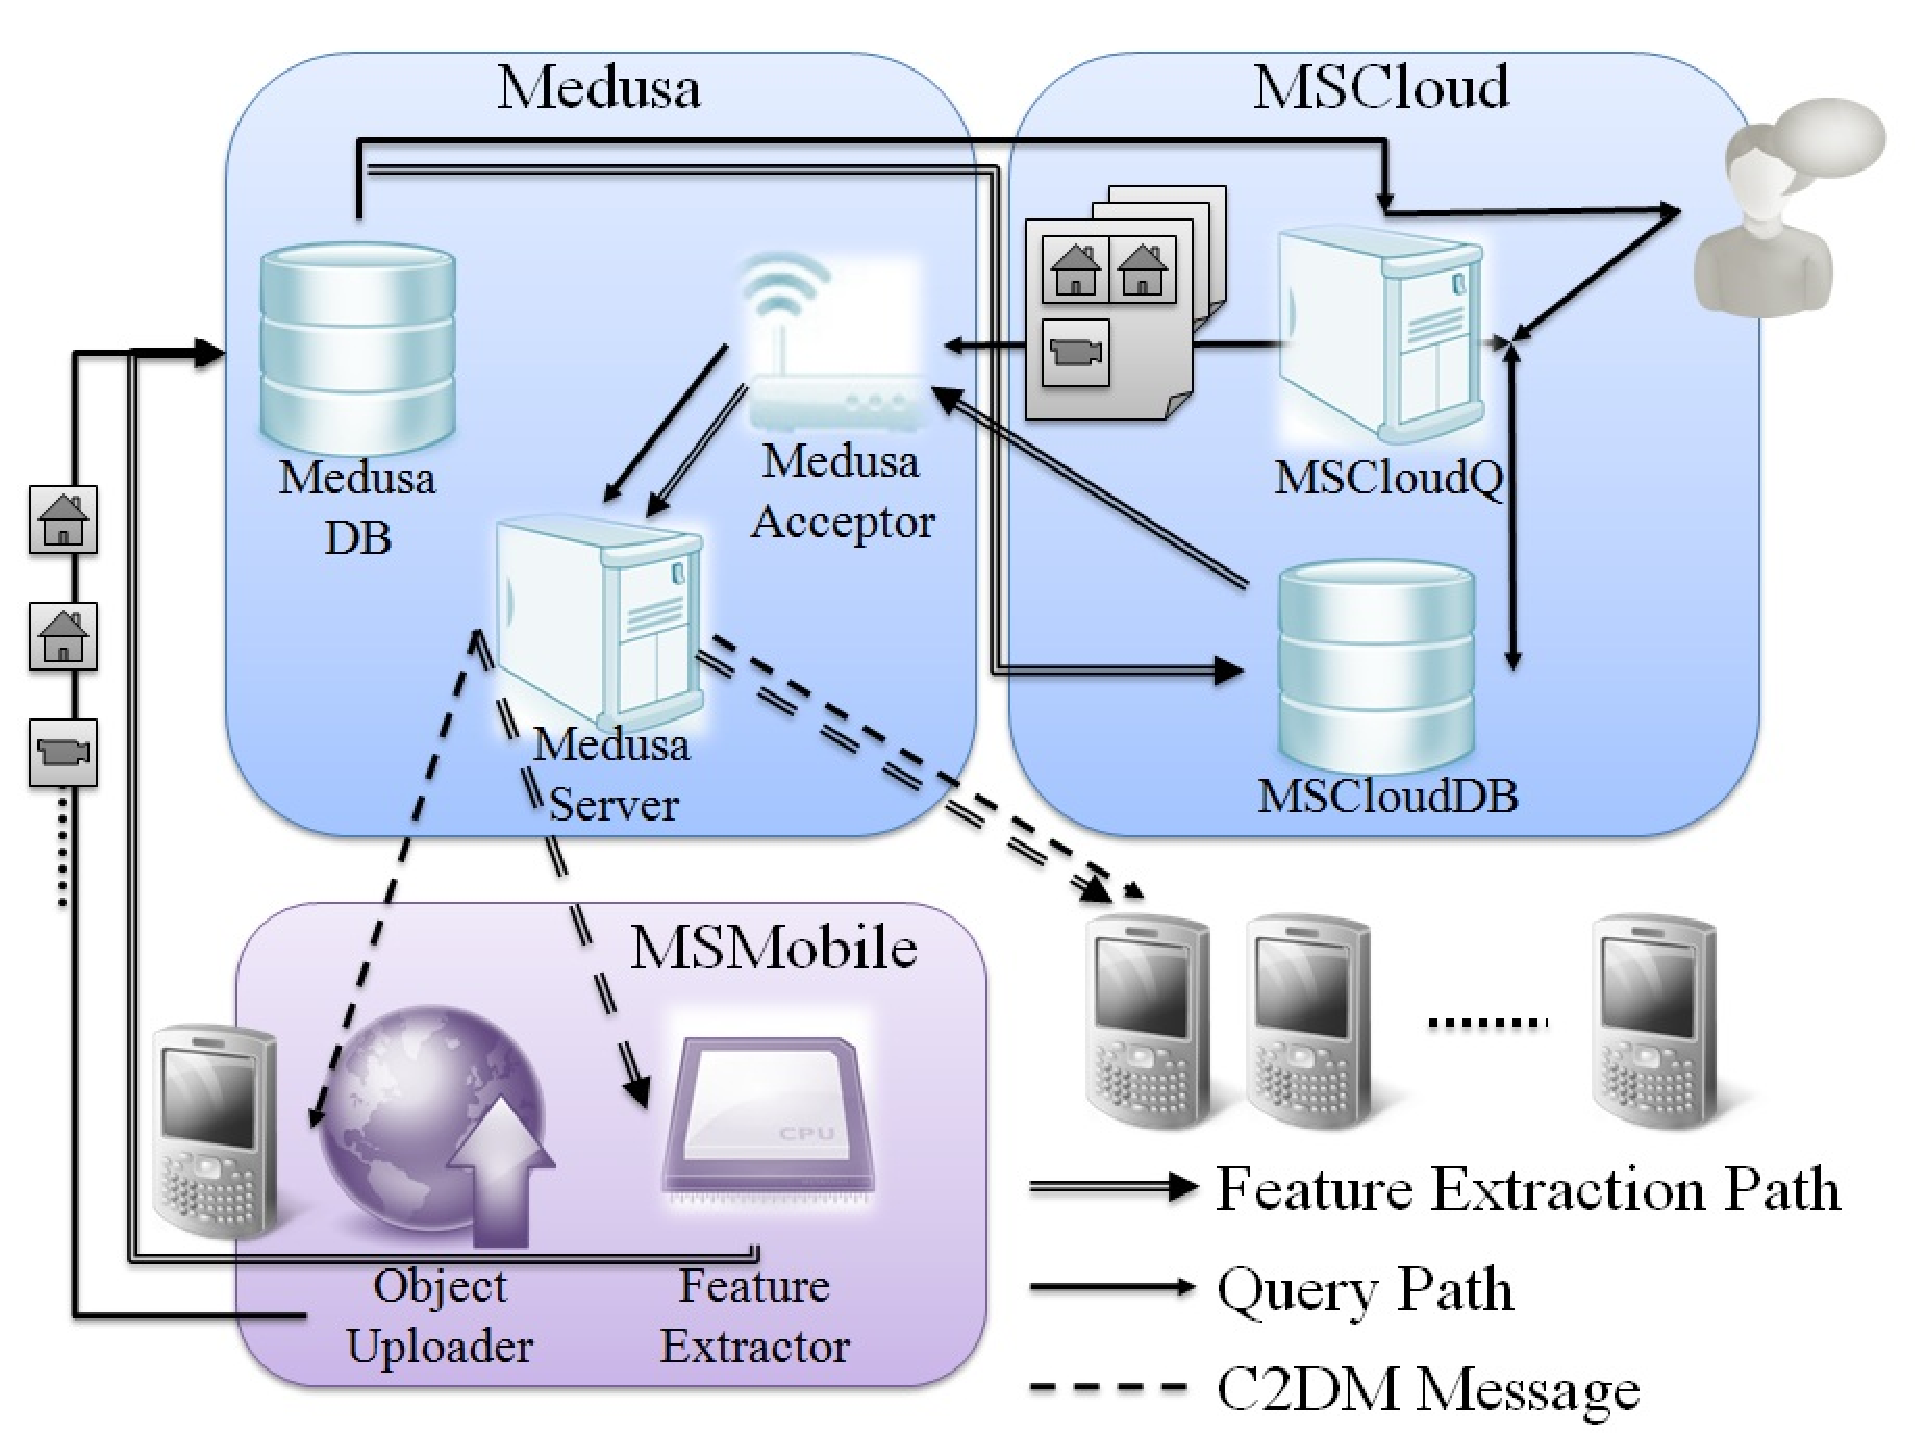
\epsfig{file=pics/architecture.eps, height=1.75in}
%\vspace{-1mm}
\caption{System architecture}
\vspace{-6mm}
\label{fig:architecture}
\end{figure}



\ignore{
In practice, file size varies since we may need to upload different type of media, such as video clips, cropped image or resized image. So the above greedy algorithm may need some modification. Current idea for this problem is to give preference to different file type, and then change the previous number bucket to size bucket so the greedy process is nearly same.

Moreover, queries usually come randomly, which raises another multi-query processing demand for the system. In this situation, we propose a dynamic scheduling adjust algorithm here. To make explanation more clear, we begin with discussion of 2-query overlap scenario, assume the first query time is $[t_{1},t_{2}]$ and second query time is $[t_{3},t_{4}]$, , so the overlapping time is $OL=[max(t_{1},t_{3}),min(t_{2},t_{4})]$, to make discussion simple, we omit the schedule computing time, and add another metric called $rank$ when assign tasks to each user. For the files in the assigned task, we give them a rank, that requires uploading the highest rank file first. The rank is given based on the average similarity, the less similarity, the higher rank, and each file in the rank is associated with a ranking value represents its similarity between other files. Let's come back to the overlap design, during the overlapping time interval $OL$, those who have overlap, should follow the 2 rules: 1. upload overlap files(files that work for both queries), 2. delete from end of 2 ranking lists based on the ranking value, until satisfies  the overlap time consumption. Now, we give a solution to 2 queries scenario, it's easy to generalize to n-query scenario-just find the overlap time interval, and delete end of ranking list until satisfy the requirement.}



\section{Vision}

Smartphones have the ability to capture high-resolution images and
video. Given the penetration of smartphones, it is now feasible to
consider crowd-sourcing searches for visual evidence in forensic
applications. For example, a police investigative unit might, after a
crime, request bystanders for crime scene images, possibly in exchange
for some financial incentives. [Add other examples?]

We envision a system in which a \emph{requester} poses a \emph{query}
for images or video. In our system, a cloud service handles the query
and extracts relevant images or video from smart phones of
participating users.

Queries may be of different types (aggregate, enumeration), and may
have timeliness requirements. More important, two aspects of this
problem space make the problem challenging:
\begin{itemize}
\item First, images from different users may be related with each
  other (e.g., may have been taken at the same time and place), and
  related images may convey less information than disparate images.
\item Second, each smartphone may have a limited ``pipe'' for sending
  images, given data plan costs as well as the fact that cellular
  network bandwidth has not kept pace with improvements in camera
  technology and smartphone storage.
\end{itemize}

To address these challenges, we consider a general framework for
crowd-sourced queries for media. In this framework, relationships
between images or videos, as determined by their metadata, is
encapsulated in an \emph{information network}. Images satisfying a
query can be determined by traversing this information
network. However, given wireless bandwidth constraints, not all of
these images can be returned as responses for the crowd search, so an
\emph{objective function} is used to determine the most relevant
queries. this objective function is constrained by a \emph{network
  model}, which codifies network bandwidth constraints.

In the next section, we give several examples of this framework.

% We focus on a timely media query application, which responds queries with media files retrieved from mobile phones. A query can be a question related to what is happening in a particular region, time range, and what is the objects the query is interested in; in other words, a query can be considered as a search condition. To answer the query, the corresponding response contains a series of related media resources, photos, video clips, audio clips, etc.

% The response should be returned within a time period, namely, the \textit{deadline} specified by the query. Since it takes some time for mobile phones to upload media files to the application server, limited media files can be delivered on time before the deadline. Different \textit{Network model}s determines different ways of uploading media files to the server. For each network model, given a uploading schedule for all the phones, it can determine whether such schedule is feasible or not, i.e., whether the uploading can be finished on time before the deadline.

% Network model gives the constraint that not any uploading schedule is feasible. Among all the feasible schedules, we want to pick the most informative and representative one to approximate the perfect response when there is no deadline constraint. \textit{Information model} determines how we define and select the best feasible uploading schedule, namely, to select a subset of media files to respond the query timely. 

\section{Example of Different Problems}

Above mentioned general framework for crowd-sourced queries can have different \emph{information model}, \emph{network model} and \emph{objective function}. In this section, we provide several examples to these three components.

\subsection{Network Model}

Network model basically defines how media files are uploaded to the application server. Due to different scenarios or applications, different network models might be used. Here we briefly describe two possible models, naive model and peer-assistant model.

\subsubsection{Naive Model}

In naive model, each mobile phone only make one connection, to the application server, and will only upload its own media files. In this model, we assume there is no interaction or interference among phones. For simplicity, we assume each phone will upload multiple media files sequentially. 

\subsubsection{Peer-Assistant Model}

For some queries with short deadline, by solely uploading its own files for each phone, the response result might not be satisfactory. If neighboring phones can help each other for uploading, it is more flexible and we can expect better response result. That is the intuition of peer-assistant model. Concretely, besides the connection to the application server, each phone can also connect to its neighboring phones through ad-hoc like links. In this case, each phone can upload its own media file as well as its neighbor's files. For example, consider an extreme case, where all the related media files are located in one phone, with strict deadline maybe only 1 photo can be uploaded; however with peer-assistant model, this phone can ask its neighbors for simultaneous uploading which might upload more files.

\subsection{Information Model}

Network model determines which uploading schedules (selection of subset of media files to upload) are feasible, while information model determines which uploading schedule is the best one. There are multiple possible information models, here we briefly discuss two models, coverage model and similarity model.

\subsubsection{Coverage Model}

The information of a media file can be represented by covered range on the physical spatial-temporal space. In other words, each media file covers some physical space. Then given a set of media files, the information such set provides is the intersection of the spaces covered by all media files. 

\subsubsection{Similarity Model}

Similarity model would not answer the provided information question directly; instead, similarity model describes the similarity between a pair of media files. In this model, given a set of media files, the information such set provides is represented by how similar each pair of media files of the subset is. Intuitively, a high averaged similarity subset of media files indicates low information, and vice versa.

\subsection{Objective Function}
\subsubsection{}

\section{Our Problem}
\label{sec:probl}

\subsection{Preliminaries}

We focus on one specific problem of the framework. In our problem we consider a cloud service, the central server and multiple participated smartphones. The query to our problem contains a feature vector (metadata) including \emph{location}, \emph{time}, \emph{number of buildings}, \emph{number of peoples}, \emph{number of cars} and \emph{photo histogram}. In addition, there is a \emph{deadline} associated with each query. 

To respond each query there are generally $4$ steps:
\begin{itemize}
\item Given the query contents, server filters out irrelevant media files and keeps the qualified ones;
\item Based on the information model and the network model, server determines uploading schedules for each participated smartphone;
\item Smartphones receives its schedule from the server, upload the media files correspondingly;
\item Server gets all the scheduled media files, responds the query.
\end{itemize}

For the first step, filtering step, we can build index based on the metadata. The index uses partial metadata as keys and sorts the all the metadatas such that for each query, qualified files can be located efficiently. Given a set of qualified files, different \emph{network model}, \emph{information model} and \emph{objective function} might determine different schedules and thus different query response. Following we define such components for our problem concretely.

\subsection{Network Model}
We consider a fairly simple network model in our problem, namely, \emph{naive model}. Assume there are $M$ participated smartphones, each of whose uploading speed is $b_{i}$. Each smartphone will upload files sequentially if there are multiple files to upload.
Each smartphone can upload files without any interference to others.

\subsection{Information Model}

We define ${similarity}$ to describe the relationship between any pair of files. To make problem clear, we take two files: file $i$ and file $j$ as an example here, the similarity vector ${\overrightarrow{v}_{i,j}}$ is composed by the following elements: time difference ${t_{i,j}}$, location difference ${d_{i,j}}$, object difference ${o_{i,j}}$, color distribution difference ${c_{i,j}}$, trace direction ${tr_{i,j}}$, etc. Since files are owned by different users, then file owner is also an important part for similarity, and we add this information as a binary value in similarity. So now we normalize these elements and define similarity as the weighted sum of these elements. With normalization, the similarity vector can be represented as follows:

 \begin{equation}
\begin{array}{l}
 {\overrightarrow{v}_{ij}} =  \\
 \left( {\frac{{{t_{i,j}}}}{{\mathop {\max }\limits_{i,j} \left( {{t_{i,j}}} \right)}},\frac{{{d_{i,j}}}}{{\mathop {\max }\limits_{i,j} \left( {{d_{i,j}}} \right)}},\frac{{{o_{i,j}}}}{{\mathop {\max }\limits_{i,j} \left( {{o_{i,j}}} \right)}},\frac{{{c_{i,j}}}}{{\mathop {\max }\limits_{i,j} \left( {{c_{i,j}}} \right)}},\frac{{t{r_{i,j}}}}{{\mathop {\max }\limits_{i,j} \left( {t{r_{i,j}}} \right)}}} \right) \\
 \end{array}
 \end{equation}



To quantify the similarity value, we define a weighted sum function for similarity vector, $f(\overrightarrow{v}_{i,j})$, which is a numerical value.

\begin{equation}
\begin{array}{l}
 f\left( {{\overrightarrow{v}_{ij}}} \right) = {\alpha _1}\frac{{{t_{i,j}}}}{{\mathop {\max }\limits_{i,j} \left( {{t_{i,j}}} \right)}} + {\alpha _2}\frac{{{d_{i,j}}}}{{\mathop {\max }\limits_{i,j} \left( {{d_{i,j}}} \right)}} +  \\
 {\alpha _3}\frac{{{o_{i,j}}}}{{\mathop {\max }\limits_{i,j} \left( {{o_{i,j}}} \right)}} + {\alpha _4}\frac{{{c_{i,j}}}}{{\mathop {\max }\limits_{i,j} \left( {{c_{i,j}}} \right)}} + {\alpha _5}\frac{{t{r_{i,j}}}}{{\mathop {\max }\limits_{i,j} \left( {t{r_{i,j}}} \right)}} \\
 \end{array}
\end{equation}

in which, $\alpha_{1}+\alpha_{2}+\alpha_{3}+\alpha_{4}+\alpha_{5}=1$, and each $\alpha$'s value is assigned by the query's preference, e.g. if commander prefers location difference, then $\alpha_{1}$ gets more percentage.

\subsection{Objective Function and Problem Formulation}

Consider the simplest case, each file is of the same size and one query scenario. After filtering, we get $N$ photos from $M$ users, each user $i$ owns $a_{i-1}$ photos, that is, $a_{0}+\ldots+a_{M-1}=N$. With the bandwidth and deadline constraint, users can only upload limited qualified files, more precisely, for user $i$, he can upload $s_{i}$ files under the constraint, in which, $s_{i}\leq a_{i}$ and $s_{0}+\ldots+s_{M-1}=K$. The problem now is to select a subset $K$ photos from these $N$ photos, such that:
\begin{equation}
\sum\limits_{i = 0}^{K - 1} {\sum\limits_{j = 0}^{K - 1} {\sum\limits_{{k_i} = 0}^{{s_i} - 1} {\sum\limits_{{k_j} = 0}^{{s_j} - 1} {f\left( {{{\vec v}_{{k_i}{k_j}}}} \right)} } } }
 \end{equation}

 get maximized, in which, $f(\overrightarrow{v}_{k_{i}k_{j}})=0$ if $k_{i}=k_{j}$ and $i=j$. 

\section{Related Works}

\subsection{Sensor Selection Problem}
Sensor selection problem focus on how to select a subset of sensors for best aggregated sensing information. 
\subsubsection{Query}
The query is to get an aggregated and overall sensing result of the entire sensor network.
\subsubsection{Objective}
Select a subset of all the sensors to get the most representative sensing results.
\subsubsection{Information Model}
Can be any information model. Actually a sensor in the sensor selection problem is exactly a media file in our problem. So any possible information model we discussed before can be applied to sensor selection problem directly.
\subsubsection{Network Model}
There is no network model for sensor selection problem, which is the main difference compared to our problem. For sensor selection problem, each sensor is a media file in our problem, which means that there is only one phone. In addition, there is no deadline constraint. So the best subset of sensors solely depends on the information model.

\subsection{PhotoNet}
\subsubsection{Query}
No specific query in this paper.
\subsubsection{Objective}
Because storage space is limited, each phone should decide the optimized photo set to store locally; namely, the stored photo set should present lowest average pairwise unsimilarity. (Based on the same idea but another minor objective is, to exchange the photo with highest unsimilarity first while encountering.)
\subsubsection{Information Model}
Use distance concept between a pair of photos, distance defined by binary geo-distance or time and color histogram. Users exchange only limited photos because of the limited meeting time and bandwidth. Peer-connection is manually.
\subsubsection{Network Model}
A typical DTN model, encounter-transmission strategy.

\subsection{PhotoNet with Outlier Elimination}
\subsubsection{Query}
Same as PhotoNet.
\subsubsection{Objective}
Same as PhotoNet, each phone is trying to maintain the most representative photo set. Instead of maximizing the distance directly, outliers are considered as the least representative photos (and will be dropped at very beginning); in the case of without any outliers, the cluster with the most number of photos will be dropped photo first, since the cluster provide redundant information.
\subsubsection{Information Model}
The distance concept is the same as above. Based on the distance, photos are grouped into clusters. The information provided by a cluster is related to how many photos are within this cluster. After ranked the photo within one cluster, as the number of photos contained in a cluster increasing, the additional information provided by the last photo (marginal utility) decreases; namely, first photo provides $p(c)$, second provides $l\cdot p(c)$, third provides $l^2\cdot p(c)$, where $l$ is a parameter which is less than $1$. A cluster with relatively small number of photos is defined as a outlier cluster.
\subsubsection{Network Model}
Same as PhotoNet.

\subsection{Diversity Caching}
\subsubsection{Query}
Same as PhotoNet.
\subsubsection{Objective}
Maximize the utility function based on the cache. The solution is simple, always drop the lowest rank item of the cluster with the maximum number of items.
\subsubsection{Information Model}
Same as "PhotoNet with Outlier Elimination", photos are grouped into clusters, the utility of the entire set is defined as the sum of the utility of all the clusters. Each cluster's utility is using the decreasing model, namely, $p(c)$, $l\cdot p(c)$, $l^2\cdot p(c)$.
\subsubsection{Network Model}
Not any.

\subsection{CrowdSearch}
\subsubsection{Query}
Query is initiated at the mobile phone, which is different from our architecture. Query is a image (query image); the server will return the images with the same contents of the query image.
\subsubsection{Objective}
Two phases photo selection for good accuracy of image response (first step is the server automatically select photos based on tags; second step is human validation).
\subsubsection{Information Model}
On the server side, all the photos are tagged automatically (SIFT). Given query image, the server will provide candidate images; after that human validation will happen on the candidates based on AMT platform.
\subsubsection{Network Model}
Delay on network communication is not important, they mainly focus on the delay of human validation of candidate images.

\subsection{TagSense}
\subsubsection{Query}
Not any.
\subsubsection{Objective}
Tag people occurred in a photo captured by smart phone automatically.
\subsubsection{Information Model}
Not any.
\subsubsection{Network Model}
Use WiFi connection to estimate distance between phones and thus tag people occurred in the photo.




%% bound, Euclidean distance, Privacy, multi parties,

{\footnotesize
\bibliographystyle{abbrv}
\bibliography{main}
}


\end{document}
